\documentclass{beamer}
\usetheme{Madrid}
\usecolortheme{seagull}
\usepackage[utf8]{inputenc}
\usepackage[russian]{babel}
\usepackage{graphicx}

% Информация о презентации
\title[Цифровая обработка звука]{Удаление артефактов. Выравнивание баланса. Восприятие звука и рекомендации по цифровой обработке. Характеристики областей звукового диапазона для восприятия. Эквалайзер. Рекомендации по обработке звука эквалайзером. Рекомендации по обработке голоса. Диапазоны частотного спектра голоса. Сжатие цифрового звука.}
\author[В. Д. Карасев]{Исполнитель: студент группы 221 факультета КНиИТ \\ В. Д. Карасев \\ Руководитель НИР: старший преподаватель М. В. Белоконь}
\institute[Саратов]{Саратовский государственный университет}
\date{Саратов, 2024}

\begin{document}

% Титульный слайд
\begin{frame}
    \titlepage
\end{frame}

% Слайд 1: Удаление артефактов и выравнивание баланса
\begin{frame}{Удаление артефактов и выравнивание баланса}
    \textbf{Удаление шумов и артефактов} Использование инструментов шумоподавления и удаления нежелательных звуков для очистки записи. \\
    \vspace{0.3cm}
    \textbf{Выравнивание баланса:} Регулировка уровней громкости различных элементов аудиозаписи для достижения сбалансированного звучания. \\
    \begin{center}
        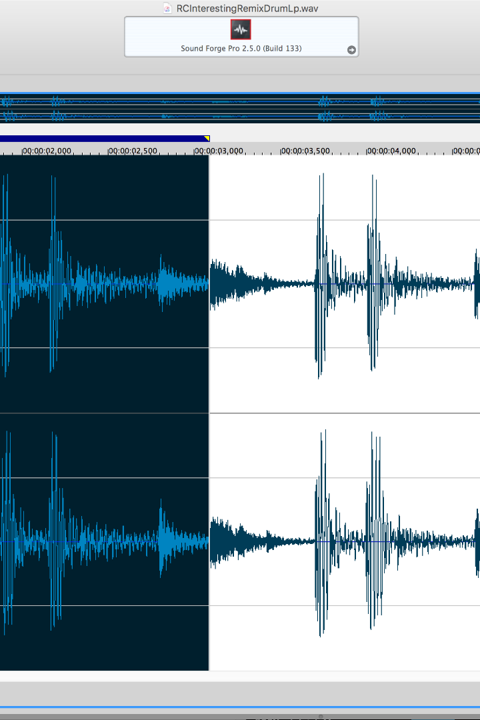
\includegraphics[width=0.6\linewidth]{pic1.png} % Замените на реальное изображение
    \end{center}
\end{frame}

% Слайд 2: Восприятие звука и рекомендации по цифровой обработке
\begin{frame}{Восприятие звука и рекомендации по цифровой обработке}
    \textbf{Восприятие Звука} Понимание того, как человеческое ухо воспринимает различные частоты и динамические диапазоны звука. \\
    \vspace{0.3cm}
    \textbf{Рекомендации по Обработке} Применение знаний о восприятии звука для оптимизации цифровой обработки и достижения желаемого звучания. \\
    \begin{center}
        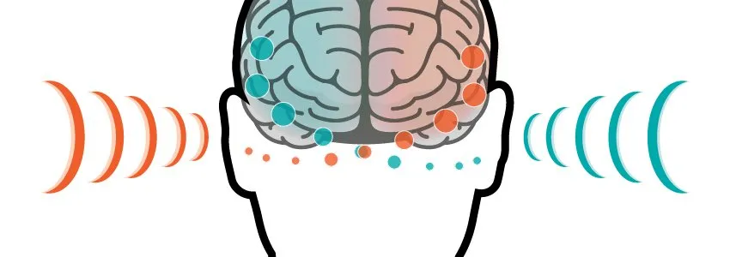
\includegraphics[width=0.6\linewidth]{pic2.png} % Замените на реальное изображение
    \end{center}
\end{frame}

% Слайд 3: Контрастные цвета
\begin{frame}{Характеристики областей звукового диапазона для восприятия}
    \textbf{Низкие Частоты: } Область от 20 Гц до 300 Гц, отвечающая за глубину и фундамент звука. \\
    \vspace{0.3cm}
    \textbf{Средние Частоты: } Область от 300 Гц до 3 кГц, ответственная за разборчивость и присутствие звука. \\
    \vspace{0.3cm}
    \textbf{Высокие Частоты: } Область от 3 кГц до 20 кГц, придающая яркость и детализацию звучанию.
    \begin{center}
        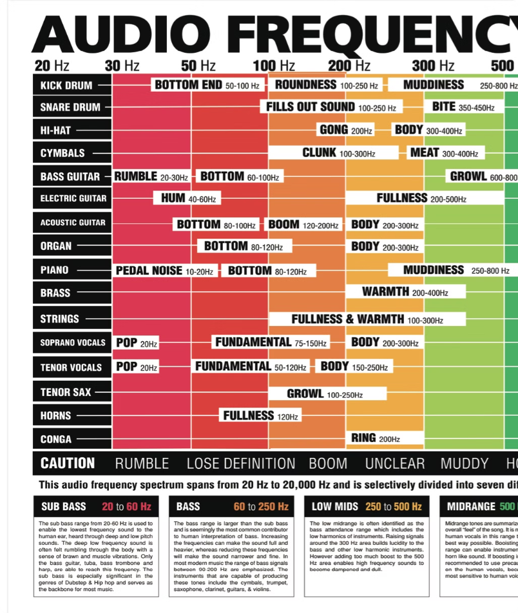
\includegraphics[width=0.6\linewidth]{pic3.png} % Замените на реальное изображение
    \end{center}
\end{frame}

% Слайд 4: Комплементарные цвета
\begin{frame}{Комплементарные цвета}
    \textbf{Определение:} Дополняют друг друга, создавая яркий контраст. \\
    \vspace{0.3cm}
    \textbf{Эффект:} Привлекают внимание и придают глубину. \\
    \vspace{0.3cm}
    \textbf{Применение:} Живопись, дизайн интерьеров.
    \begin{center}
        \includegraphics[width=0.6\linewidth]{complementary_example.png} % Замените на реальное изображение
    \end{center}
\end{frame}

% Слайд 5: Триадные гармонические схемы
\begin{frame}{Триадные гармонические схемы}
    \textbf{Выбор цветов:} Три цвета, равномерно расположенные на цветовом круге. \\
    \vspace{0.3cm}
    \textbf{Эффект:} Динамическое равновесие, выразительные композиции. \\
    \vspace{0.3cm}
    \textbf{Применение:} Логотипы для передачи разнообразия.
    \begin{center}
        \includegraphics[width=0.6\linewidth]{triadic_example.png} % Замените на реальное изображение
    \end{center}
\end{frame}

% Слайд 6: Источники
\begin{frame}{Список использованных источников}
    \begin{itemize}
        \item Опенгейм А. В., Шафер Р. В. Цифровая обработка сигналов. Мир, 1979.
        \item Дмитриев В. А. Цифровая обработка сигналов: Учебное пособие. Лаборатория знаний, 2013.
        \item Мюллер М. Fundamentals of Music Processing: Audio, Analysis, Algorithms, Applications. Springer, 2015.
        \item Рэбинар Л., Голд Б. Теория и применение цифровой обработки сигналов. Мир, 1978.
    \end{itemize}
\end{frame}

% Слайд 7: Спасибо за внимание
\begin{frame}
    \centering
    \textbf{\huge Спасибо за внимание!}
\end{frame}

\end{document}
